%% -*- mode: LaTeX; coding: utf-8; -*-
\documentclass[tikz]{standalone}

\usepackage{tikz}
\usetikzlibrary{arrows,shapes}

\begin{document}

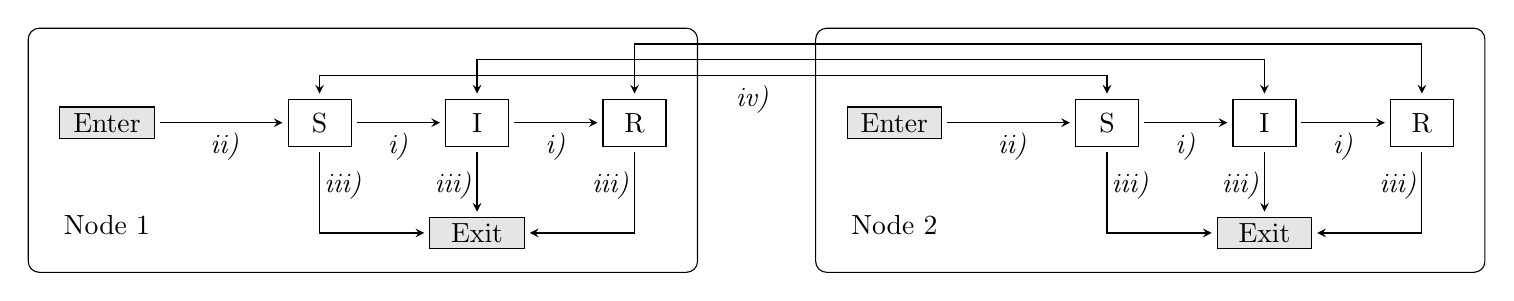
\begin{tikzpicture}[node distance=1ex]
  \draw[rounded corners] (0,3.4) rectangle (8.5,6.5);
  \draw[rounded corners] (10,3.4) rectangle (18.5,6.5);

  \node at (1,4) {Node 1};
  \node at (11,4) {Node 2};

  %% Compartments
  \draw (3.3,5) rectangle (4.1,5.6);
  \node at (3.7,5.3) {S};
  \draw (13.3,5) rectangle (14.1,5.6);
  \node at (13.7,5.3) {S};
  \draw (5.3,5) rectangle (6.1,5.6);
  \node at (5.7,5.3) {I};
  \draw (15.3,5) rectangle (16.1,5.6);
  \node at (15.7,5.3) {I};
  \draw (7.3,5) rectangle (8.1,5.6);
  \node at (7.7,5.3) {R};
  \draw (17.3,5) rectangle (18.1,5.6);
  \node at (17.7,5.3) {R};

  \draw [fill=black!10] (0.4,5.1) rectangle (1.6,5.5);
  \node at (1,5.3) {Enter};
  \draw [fill=black!10] (10.4,5.1) rectangle (11.6,5.5);
  \node at (11,5.3) {Enter};

  \draw[>=stealth,shorten <=2pt, shorten >=2pt,->]
  (1.6,5.3) to (3.3,5.3);
  \draw[>=stealth,shorten <=2pt, shorten >=2pt,->]
  (11.6,5.3) to (13.3,5.3);
  \node at (2.5,5) {\textit{ii)}};
  \node at (12.5,5) {\textit{ii)}};

  \draw [fill=black!10] (5.1,3.7) rectangle (6.3,4.1);
  \node at (5.7,3.9) {Exit};
  \draw [fill=black!10] (15.1,3.7) rectangle (16.3,4.1);
  \node at (15.7,3.9) {Exit};

  %% Gillespie
  \draw[>=stealth,shorten <=2pt, shorten >=2pt,->]
  (4.1,5.3) to (5.3,5.3);
  \draw[>=stealth,shorten <=2pt, shorten >=2pt,->]
  (6.1,5.3) to (7.3,5.3);
  \draw[>=stealth,shorten <=2pt, shorten >=2pt,->]
  (14.1,5.3) to (15.3,5.3);
  \draw[>=stealth,shorten <=2pt, shorten >=2pt,->]
  (16.1,5.3) to (17.3,5.3);
  \node at (4.7,5) {\textit{i)}};
  \node at (6.7,5) {\textit{i)}};
  \node at (14.7,5) {\textit{i)}};
  \node at (16.7,5) {\textit{i)}};

  %% External transfer events
  \draw[>=stealth,shorten <=2pt, shorten >=2pt,<->]
  (3.7,5.6) to (3.7,5.9) to (13.7,5.9) to (13.7,5.6);
  \draw[>=stealth,shorten <=2pt, shorten >=2pt,<->]
  (5.7,5.6) to (5.7,6.1) to (15.7,6.1) to (15.7,5.6);
  \draw[>=stealth,shorten <=2pt, shorten >=2pt,<->]
  (7.7,5.6) to (7.7,6.3) to (17.7,6.3) to (17.7,5.6);
  \node at (9.2,5.6) {\textit{iv)}};

  %% Exit events
  \draw[>=stealth,shorten <=2pt, shorten >=2pt,->]
  (3.7,5) to (3.7,3.9) to (5.1,3.9);
  \draw[>=stealth,shorten <=2pt, shorten >=2pt,->]
  (5.7,5) to (5.7,4.1);
  \draw[>=stealth,shorten <=2pt, shorten >=2pt,->]
  (7.7,5) to (7.7,3.9) to (6.3,3.9);
  \draw[>=stealth,shorten <=2pt, shorten >=2pt,->]
  (13.7,5) to (13.7,3.9) to (15.1,3.9);
  \draw[>=stealth,shorten <=2pt, shorten >=2pt,->]
  (15.7,5) to (15.7,4.1);
  \draw[>=stealth,shorten <=2pt, shorten >=2pt,->]
  (17.7,5) to (17.7,3.9) to (16.3,3.9);
  \node at (4,4.5) {\textit{iii)}};
  \node at (5.4,4.5) {\textit{iii)}};
  \node at (7.4,4.5) {\textit{iii)}};
  \node at (14,4.5) {\textit{iii)}};
  \node at (15.4,4.5) {\textit{iii)}};
  \node at (17.4,4.5) {\textit{iii)}};

\end{tikzpicture}

\end{document}
